\section{Übung - OLAP}
\label{sec:uebung_06}

% ##########################################################################
% ############################### Aufgabe 01 ###############################
% ##########################################################################
\subsection{Aufgabe}
\label{sec:uebung_06.aufgabe_01}
Erzeuge folgende Übersicht über die Anzahl der Mitarbeiter in jeder Abteilung, in jeder Stadt und in jedem Land.

\begin{figure}[H]
  \centering
  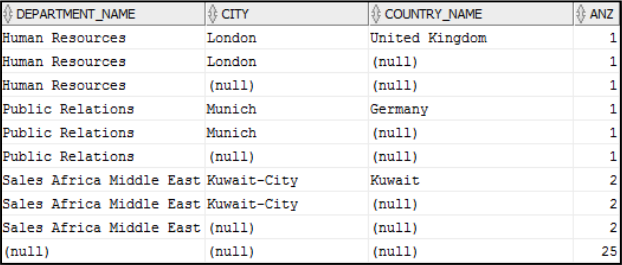
\includegraphics[width=1\textwidth]{img//uebung_06_-_aufgabe_01.png}
  \label{img:uebung_06_-_aufgabe_01}
\end{figure}

\subsubsection*{Lösung}
\label{sec:uebung_06.aufgabe_01.loesung}
\inputsql{./loesungen/uebung_06/uebung_06_-_aufgabe_01.sql}


% ##########################################################################
% ############################### Aufgabe 02 ###############################
% ##########################################################################
\subsection{Aufgabe}
\label{sec:uebung_06.aufgabe_02}
Zur Übersicht der Mitarbeitergehälter soll folgende Ausgabe mittels geeigneter Gruppierung erreicht werden.


\begin{table}[H]
  \centering
  \ttfamily
  \small
  \begin{tabular}{|l|l|l|l|l|}
    \hline
    \textbf{CITY}  & \textbf{DEPARTMENT} & \textbf{JOB}         & \textbf{NAME}  & \textbf{SALARY}  \\
    \hline
    London         & Human Resources     & \textit{-all-}       & Susan Mavris   & 6500             \\
    London         & Human Resources     & \textit{-all-}       & \textit{-all-} & 6500             \\
    London         & \textit{-all-}      & \textit{-all-}       & \textit{-all-} & 6500             \\
    Munich         & Public Relations    & \textit{-all-}       & Hermann Baer   & 10000            \\
    Munich         & Public Relations    & \textit{-all-}       & \textit{-all-} & 10000            \\
    Munich         & \textit{-all-}      & \textit{-all-}       & \textit{-all-} & 10000            \\
    Oxford         & Sales Europe        & \textit{-all-}       & David Lee      & 6800             \\
    Oxford         & Sales Europe        & \textit{-all-}       & Lisa Ozer      & 11500            \\
    Oxford         & Sales Europe        & \textit{-all-}       & Amit Banda     & 6200             \\
    Oxford         & Sales Europe        & \textit{-all-}       & Ellen Abel     & 11000            \\
    $[$\dots$]$    & $[$\dots$]$         & $[$\dots$]$          & $[$\dots$]$    & $[$\dots$]$          \\
    \textit{-all-} & \textit{-all-}      & Sales Representative & \textit{-all-} & 1157485          \\
    \textit{-all-} & \textit{-all-}      & Shipping Clerk       & \textit{-all-} & 64300            \\
    \textit{-all-} & \textit{-all-}      & Stock Clerk          & \textit{-all-} & 55700            \\
    \textit{-all-} & \textit{-all-}      & Stock Manager        & \textit{-all-} & 36400            \\
    \textit{-all-} & \textit{-all-}      & \textit{-all-}       & \textit{-all-} & 1598401          \\
    \hline
  \end{tabular}
\end{table}

\subsubsection*{Lösung}
\label{sec:uebung_06.aufgabe_02.loesung}
\inputsql{./loesungen/uebung_06/uebung_06_-_aufgabe_02.sql}


% ##########################################################################
% ############################### Aufgabe 03 ###############################
% ##########################################################################
\subsection{Aufgabe}
\label{sec:uebung_06.aufgabe_03}
Die Vertriebsabteilung benötigt eine Auswertung über den Umsatz zwischen 2010 und 2012 insgesamt, je Jahr, je Land und Region sowie je Jahr, Land und Region.

\begin{table}[H]
  \centering
  \ttfamily
  \begin{tabular}{|l|l|l|l|}
    \hline
    \textbf{YEAR} & \textbf{COUNTRY} & \textbf{REGION}        & \textbf{SALES}  \\
    \hline
    2010          & China            & Asia                   & 4892716         \\
    2011          & China            & Asia                   & 3056097         \\
    2012          & China            & Asia                   & 4359027         \\
    2010          & Egypt            & Middle East and Africa & 3866210         \\
    2011          & Egypt            & Middle East and Africa & 4397054         \\
    2012          & Egypt            & Middle East and Africa & 3525384         \\
    $[$\dots$]$   &                  &                        &                 \\
                  & China            & Asia                   & 12307840        \\
                  & Egypt            & Middle East and Africa & 11788648        \\
    $[$\dots$]$   &                  &                        &                 \\
    2010          &                  &                        & 125719979       \\
    2011          &                  &                        & 114614129       \\
    2012          &                  &                        & 124466612       \\
                  &                  &                        & 364800720       \\
    \hline
  \end{tabular}
\end{table}

\subsubsection*{Lösung}
\label{sec:uebung_06.aufgabe_03.loesung}
\inputsql{./loesungen/uebung_06/uebung_06_-_aufgabe_03.sql}


% ##########################################################################
% ############################### Aufgabe 04 ###############################
% ##########################################################################
\subsection{Aufgabe}
\label{sec:uebung_06.aufgabe_04}
Geben Sie für jeden Job, die Anzahl der Mitarbeiter in den Ländern 'United Kingdom', 'United States of America', 'Germany', 'Kuwait', 'Canada' und 'Singapore' in einer Zeile aus.

\begin{figure}[H]
  \centering
  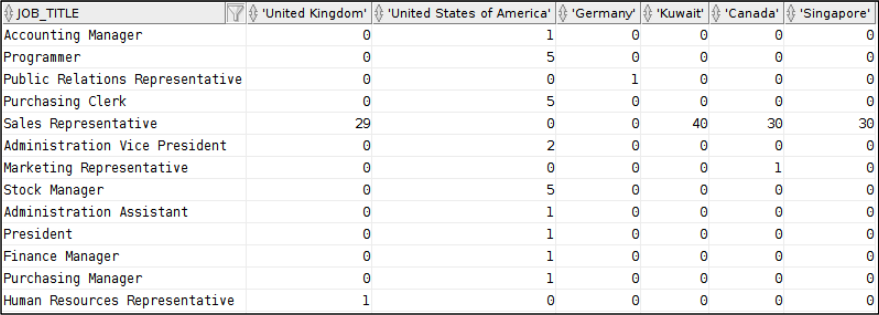
\includegraphics[width=1\textwidth]{img//uebung_06_-_aufgabe_04.png}
  \label{img:uebung_06_-_aufgabe_04}
\end{figure}

\subsubsection*{Lösung}
\label{sec:uebung_06.aufgabe_04.loesung}
\inputsql{./loesungen/uebung_06/uebung_06_-_aufgabe_04.sql}
